% Journal of Bioinformatics and Computational Biology submission source.
% Uses the unmodified author-supplied World Scientific class dated 2026/05/18.
\pdfminorversion=7
\pdfsuppresswarningpagegroup=1
\documentclass{ws-jbcb}

\usepackage[super]{cite}
\usepackage{xcolor}
\usepackage[verbose,hypertexnames=false]{hyperref}
\hypersetup{colorlinks=false,allbordercolors=blue,pdfborderstyle={/S/U/W 1}}
\usepackage{array}
\usepackage{tabularx}
\usepackage{xurl}

\graphicspath{{./}{../../figs/}}

% theorem, proposition, definition, example, remark, and proof are class-native.
\newtheorem{algorithm}{Algorithm}
\numberwithin{equation}{section}

\newcommand{\tas}{\textit{Arabidopsis thaliana}}
\newcommand{\ath}{\textit{A.\ thaliana}}
\newcommand{\hs}{\textit{Homo sapiens}}
\newcommand{\TAU}{\tau}
\newcommand{\xRightarrow}[1]{\stackrel{#1}{\Longrightarrow}}
\newcommand{\LTS}{\mathcal{L}}
\newcommand{\powerset}{\mathcal{P}}
\newcommand{\strongsim}{\mathrel{\sim_{s}}}
\newcommand{\weaksim}{\mathrel{\sim_{w}}}
\newcommand{\weakpre}{\mathrel{\preceq_{w}}}
\newcolumntype{Y}{>{\raggedright\arraybackslash}X}

\hypersetup{
  pdftitle={A formal and reproducible framework for auditing observable behavior in qualitative biological network models},
  pdfauthor={Carlos Ramirez Ovalle},
  pdfkeywords={qualitative biological networks, Petri nets, labeled transition systems, weak bisimulation, model checking, Boolean networks}
}

\begin{document}

\markboth{C. Ramirez Ovalle}{Formal and reproducible audit of biological network models}
\catchline{}{}{}{}{}

\title{A formal and reproducible framework for auditing observable behavior in
qualitative biological network models}

\author{Carlos Ramirez Ovalle\footnote{Corresponding author.}}

\address{Department of Natural Sciences and Mathematics, Pontificia Universidad
Javeriana Cali, Calle 18 No. 118-250, Via a Pance, Cali, Valle del Cauca,
Colombia\\
carlosovalle@javerianacali.edu.co}

\maketitle

\begin{abstract}
Structurally similar qualitative biological networks can differ in reachable
branching, whereas mechanistically different models may agree when internal
events are hidden. We map Petri nets and logical models to finite reachable
labeled transition systems and classify strong/weak bisimilarity, directional
weak simulation, or non-comparability under a declared interface. We prove
correctness and termination for finite systems. Six construction-level controls
served only as software verification: weak bisimulation recovered 6/6 decisions,
and Python and mCRL2 agreed on 42 strong/weak decisions. The central case asks
where encoded animal/human and \textit{Arabidopsis} DNA-damage responses retain
common control behavior. Their unchanged structures scored 0.9976 by PN-GDDA.
Coarse and pathway-resolved interfaces were weakly bisimilar; a
mechanism-resolved interface distinguishing mammalian apoptosis from plant SMR
and differentiation/endoreduplication became non-comparable ($d_6=0.353$). This
locates a model-derived boundary between shared function and mechanism-specific
behavior without implying organism-level equivalence. In an exploratory
HPN-DREAM analysis, nine directional relations were retained without ordinal
encoding; associations and the CASPOTS native-context advantage were
inconclusive (exact $p=0.25$). Structural and behavioral comparisons therefore
provide complementary, interface-conditional evidence.
\end{abstract}

\keywords{Qualitative biological networks; Petri nets; labeled transition
systems; weak bisimulation; model checking; Boolean networks.}

\section{Introduction}\label{sec:introduction}

Qualitative biological networks make regulatory and signaling assumptions
executable when kinetic information is unavailable or deliberately abstracted.
Models intended to represent related functions may nevertheless come from
different organisms, formalisms, curation choices, or update semantics. A useful
comparison must therefore ask not only whether their graphs look alike, but
whether their reachable executions preserve the biological events and choices
relevant to a stated question. Petri nets represent causality, conflict, and
concurrency explicitly, whereas logical models encode discrete regulatory
rules.\cite{Murata1989,ChaouiyaPetriBio2007,Li2006,Fisher2007}

Structural similarity does not determine observable executable behavior.
Graphlet methods sensitively compare local motifs; PN-GDDA, for example, uses
151 directed bipartite Petri-net graphlets and 592 published orbit
slots.\cite{Szawulak2022} By design, that score does not encode transition
labels, initial marking, or recursively reachable branching. Conversely,
internal refinement can alter topology without changing behavior visible at a
chosen interface. Structural and behavioral comparisons consequently answer
different, complementary questions.

This distinction is biological as well as technical. Animal/human and plant
DNA-damage responses share high-level functions such as lesion sensing,
checkpoint activation, repair, and recovery, but implement regulation and
terminal responses differently. Mammalian networks include p53-associated
checkpoint and apoptotic programs, whereas \tas{} uses the plant-specific SOG1
network, WEE1 and SMR checkpoint regulators, and damage-associated
differentiation or endoreduplication responses.\cite{JacksonBartek2009,
BlackfordJackson2017,Yoshiyama2013,DeSchutter2007,Yi2014,Adachi2011}
The resulting modeling question is resolution-dependent: at what biological
level do the two encoded control structures preserve the same observable
behavior, and when do mechanism-specific outcomes make that correspondence
fail? The set of observable labels, denoted by $\Sigma$, is therefore treated as
a biological hypothesis to be declared and tested rather than a neutral
software option.

Linear traces add event order but omit where alternatives become committed.
Two models can generate the same finite sequences while resolving a biological
choice at different states. Branching-time equivalences retain that information,
and simulation preorders report asymmetric containment when every behavior of one
model can be matched by another. Recent formal work on asynchronous Boolean
networks likewise highlights the role of reachability and branching structure in
phenotypic analysis.\cite{Yizengaw2026}

Let $N_1$ and $N_2$ be executable labeled models and let $\Sigma$ be a declared
observable interface. We formulate the comparison as
\begin{equation}\label{eq:comparison-map}
 (N_1,N_2,\Sigma)
 \longmapsto (\LTS(N_1),\LTS(N_2))
 \longmapsto C_{\Sigma}(\LTS(N_1),\LTS(N_2)),
\end{equation}
where $\LTS(N_i)$ is the finite reachable labeled transition system and
$C_{\Sigma}$ returns the strongest supported class among strong bisimilarity,
weak bisimilarity, mutual weak simulation, either one-way weak simulation, and
non-comparability. We call the reporting priority \emph{graded}: a stronger
relation suppresses weaker implied labels. This is an implication-aware
classifier, not an algebraic grading. Structural and truncated-trace measures
remain attached diagnostics rather than substitutes for $C_{\Sigma}$.

The formal relations are standard, but their application is made auditable. We
define the observable interface and simulation orientation, prove
greatest-fixed-point correctness for the executed relation-deletion algorithm,
and establish the hierarchy supporting the classifier. Controlled silent
refinement and minimal counterexamples separate structure, traces, and
branching. Construction-level cases, mCRL2, and an independently coded
attacker--defender game verify implementation behavior; they are not presented
as biological validation.

The biological application is organized around the GIM DNA-damage case. Three
interfaces fixed from the model definitions and literature range from coarse
function to mechanism-resolved terminal fate; the model structures are held
constant. A secondary RCD case illustrates directional containment. Public
GINsim controls test SBML-qual/GINML ingestion and update semantics, not
biological truth.\cite{Naldi2018,Chaouiya2013SBML,Traynard2016,
AbouJaoude2009} Finally, nine HPN-DREAM/CASPOTS pair--condition observations
show how formal outputs can be confronted with held-out perturbation data, but
the analysis is explicitly exploratory.\cite{Hill2016,Razzaq2018}

The contributions are:
\begin{romanlist}[(iv)]
\item a formal bioinformatics framework that audits two executable qualitative
biological models under a declared interface;
\item mathematical guarantees for the implemented classifier, together with
properties and counterexamples distinguishing structure, traces, and branching;
\item independent formal/software verification through six controlled cases,
mCRL2, 67,600 attacker--defender comparisons, regression tests, and observed
computational scaling; and
\item a multi-interface GIM analysis that separates high-level encoded
correspondence from organism-specific terminal behavior, with supporting public
model controls and an exploratory held-out HPN analysis.
\end{romanlist}

Throughout, four evidence layers are kept separate: formal correctness,
software/implementation verification, support for executable model construction
and ingestion, and independent biological evidence or interpretation. PN-GDDA
and the structural profile summarize topology; traces retain order but not the
location of choices; LTS-GDA retains labeled local motifs; bisimulation and
simulation match recursive branching. None of these formal outputs alone
establishes that a curated model is experimentally valid.

The operational sequence is summarized in Fig.~\ref{fig:pipeline}. Biological
question and interface declaration precede formal encoding, reachability, and
classification, making the abstraction assumptions inspectable before an
equivalence calculation is interpreted.

\begin{figure}[t]
\centering
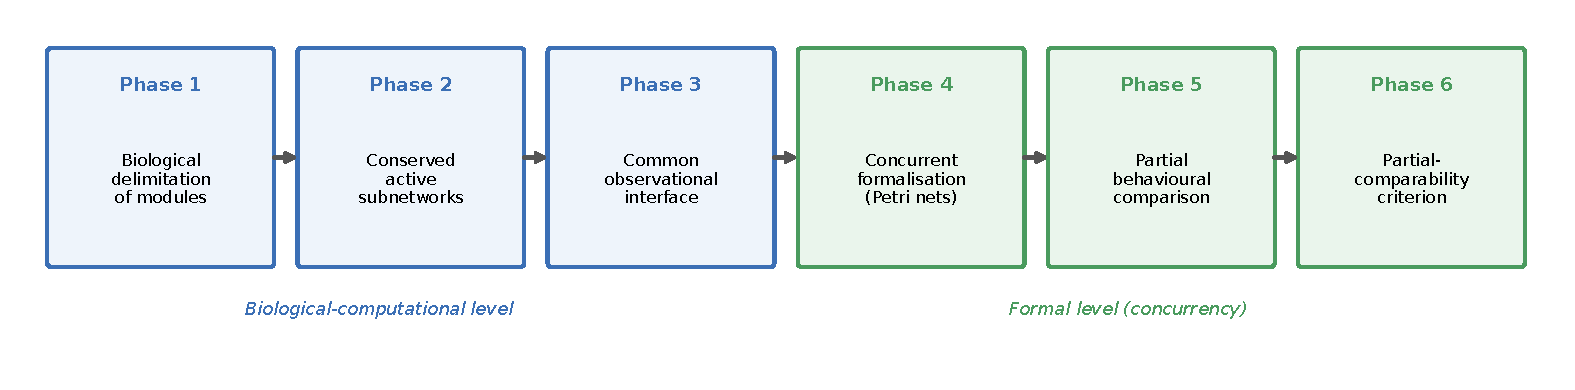
\includegraphics[width=0.96\textwidth]{Fig1.pdf}
\caption{Six-stage workflow. Stages 1--3 delimit the model-comparison question
and observational interface; stages 4--6 construct executable Petri nets,
compare their reachable behavior, and assign a model-level relation.}
\label{fig:pipeline}
\alttext{A six-stage workflow from biological question and observable interface
through formal encoding, reachable-state construction, and model comparison.}
\end{figure}

\section{Formal framework for observable biological-model comparison}
\label{sec:framework}

\subsection{Labeled Petri nets and induced transition systems}
\label{sec:petri}

\begin{definition}[Labeled place/transition net]\label{def:petri-net}
A labeled place/transition net is a tuple
\begin{equation}\label{eq:petri-net}
 N=(P,T,\operatorname{pre},\operatorname{post},\ell,m_0),
\end{equation}
where $P$ and $T$ are finite sets of places and transitions,
$\operatorname{pre},\operatorname{post}:T\to\mathbb{N}^{P}$ are the input and
output multisets, $m_0\in\mathbb{N}^{P}$ is the initial marking, and
$\ell:T\to\Sigma\cup\{\TAU\}$ assigns either an observable action in the declared
interface $\Sigma$ or the internal action $\TAU$.
\end{definition}

Under standard interleaving semantics, $t$ is enabled at $m$ when
$\operatorname{pre}(t)\leq m$ componentwise; firing it changes $m$ to
$m-\operatorname{pre}(t)+\operatorname{post}(t)$. The implementation uses
a worklist to enumerate reachable markings explicitly. A state cap and a token
bound make failure to establish a finite state space explicit rather than silently
truncating the relation calculation. All curated Petri nets used in Section
\ref{sec:applications} are safe, but the definitions below apply to every finite
reachable system.

\begin{definition}[Finite labeled transition system]\label{def:lts}
A finite labeled transition system (LTS) is
\begin{equation}\label{eq:lts}
 L=(S,\Sigma_{\TAU},\longrightarrow,s_0),\qquad
 \Sigma_{\TAU}=\Sigma\cup\{\TAU\},
\end{equation}
where $S$ is a finite state set, $s_0\in S$, and
$\longrightarrow\;\subseteq S\times\Sigma_{\TAU}\times S$. We write
$s\xrightarrow{a}s'$ for $(s,a,s')\in\longrightarrow$. The reachable semantics
of the net in Definition \ref{def:petri-net} is denoted by $\LTS(N)$.
\end{definition}

\subsection{Observable and weak transitions}\label{sec:weak-transitions}

\begin{definition}[Silent closure and weak target sets]\label{def:weak-move}
For $s\in S$, let
\begin{equation}\label{eq:tau-closure}
 \operatorname{Cl}_{\TAU}(s)=
 \{u\in S:s\xrightarrow{\TAU *}u\}.
\end{equation}
For $a\in\Sigma$, define
\begin{equation}\label{eq:weak-target}
 W_a(s)=\{v:\exists u,w\quad
 s\xrightarrow{\TAU *}u\xrightarrow{a}w\xrightarrow{\TAU *}v\},
 \qquad W_{\TAU}(s)=\operatorname{Cl}_{\TAU}(s).
\end{equation}
We write $s\xRightarrow{a}v$ when $v\in W_a(s)$.
\end{definition}

The convention $W_{\TAU}=\operatorname{Cl}_{\TAU}$ is important: a direct silent
move on one side may be matched by zero or more silent moves on the other. It is
also the convention implemented by the Python engine and used in the AUT exports
checked by mCRL2.

\subsection{Simulation and bisimulation}\label{sec:relations}

Let $L_i=(S_i,\Sigma_{\TAU},\longrightarrow_i,s_i^0)$ for $i\in\{1,2\}$.

\begin{definition}[Weak simulation]\label{def:weak-simulation}
A relation $R\subseteq S_1\times S_2$ is a weak simulation from $L_1$ to $L_2$
if, whenever $(x,y)\in R$ and $x\xrightarrow{a}_1x'$, there is
$y'\in W_a^2(y)$ such that $(x',y')\in R$. We write
\begin{equation}\label{eq:simulation-orientation}
 L_1\weakpre L_2
\end{equation}
if $(s_1^0,s_2^0)$ belongs to some such relation. Thus the right-hand system
$L_2$ simulates the left-hand system $L_1$; the left-hand behavior is contained
in the right-hand behavior under the interface.
\end{definition}

\begin{definition}[Weak and strong bisimulation]\label{def:bisimulation}
A relation $R\subseteq S_1\times S_2$ is a weak bisimulation if it satisfies the
condition in Definition \ref{def:weak-simulation} and, for every $(x,y)\in R$ and
$y\xrightarrow{a}_2y'$, there is $x'\in W_a^1(x)$ with $(x',y')\in R$. The
initial systems are weakly bisimilar, written $L_1\weaksim L_2$, when their
initial pair belongs to such a relation. Strong bisimulation, written
$L_1\strongsim L_2$, replaces every weak target set $W_a^i(x)$ by the direct
target set $\{x':x\xrightarrow{a}_i x'\}$, including for $a=\TAU$.
\end{definition}

These are standard branching-time relations.\cite{Milner1989,Sangiorgi2011}
The explicit orientation in \eqref{eq:simulation-orientation} prevents the common
ambiguity between ``simulates'' and ``is simulated by'' in one-way results.

\subsection{Weak trace language}\label{sec:trace-language}

\begin{definition}[Exact and truncated weak traces]\label{def:weak-traces}
The finite weak observable language of $L$ is
\begin{equation}\label{eq:exact-language}
 L_w(L)=\{a_1\cdots a_r\in\Sigma^*:s_0
 \xRightarrow{a_1}\cdots\xRightarrow{a_r}s
 \text{ for some }s\in S\}.
\end{equation}
Its depth-$k$ restriction is
$L_{\leq k}(L)=\{u\in L_w(L):|u|\leq k\}$. The diagnostic distance is
\begin{equation}\label{eq:distance}
d_k(L_1,L_2)=1-
\frac{|L_{\leq k}(L_1)\cap L_{\leq k}(L_2)|}
{|L_{\leq k}(L_1)\cup L_{\leq k}(L_2)|}.
\end{equation}
\end{definition}

The implementation computes the prefix-closed truncated sets in Definition
\ref{def:weak-traces}. The statement $d_k=0$ is therefore not identified with
exact weak-trace equivalence. Exact weak-trace results in this study come only
from mCRL2 or from a finite construction for which the complete language is
enumerated analytically.

\subsection{Graded behavioral classification}\label{sec:decision}

\begin{definition}[Graded classifier]\label{def:classifier}
For finite $L_1,L_2$ over the declared interface $\Sigma$, define
$C_{\Sigma}(L_1,L_2)$ by the following priority:
\begin{equation}\label{eq:classifier}
C_{\Sigma}(L_1,L_2)=
\begin{cases}
\mathsf{strong}, & L_1\strongsim L_2,\\
\mathsf{weak}, & L_1\not\strongsim L_2\text{ and }L_1\weaksim L_2,\\
\mathsf{mutual}, & L_1\not\weaksim L_2,\ L_1\weakpre L_2,\ L_2\weakpre L_1,\\
\mathsf{left\_in\_right}, & L_1\weakpre L_2,\ L_2\not\weakpre L_1,\\
\mathsf{right\_in\_left}, & L_2\weakpre L_1,\ L_1\not\weakpre L_2,\\
\mathsf{noncomparable}, & \text{otherwise}.
\end{cases}
\end{equation}
The output is a reporting class, not a newly proposed equivalence relation.
\end{definition}

\begin{proposition}[Exclusive reporting]\label{prop:classifier}
The classifier in Definition \ref{def:classifier} assigns exactly one class to
every ordered pair of finite LTSs.
\end{proposition}

\begin{proof}
The first two cases are selected before any simulation-only case. If neither is
selected, the two simulation predicates have exactly four Boolean combinations:
both true, only the first true, only the second true, or both false. These are the
last four cases of \eqref{eq:classifier}, respectively. The cases are exhaustive
and disjoint by their stated guards.
\end{proof}

\subsection{Fixed-point computation and formal properties}
\label{sec:fixed-point}

For $a\in\Sigma_{\TAU}$, let $D_a^i(x)=\{x':x\xrightarrow{a}_i x'\}$ and
$U=S_1\times S_2$. Define operators on $\powerset(U)$ by
\begin{align}
\Phi_{\preceq}(R)=\{(x,y)\in U:
 &\ \forall a,x'\in D_a^1(x)\ \exists y'\in W_a^2(y),
 (x',y')\in R\},\label{eq:sim-operator}\\
\Phi_w(R)=\{(x,y)\in\Phi_{\preceq}(R):
 &\ \forall a,y'\in D_a^2(y)\ \exists x'\in W_a^1(x),
 (x',y')\in R\},\label{eq:weak-bisim-operator}\\
\Phi_s(R)=\{(x,y)\in U:
 &\ \forall a,x'\in D_a^1(x)\ \exists y'\in D_a^2(y),
 (x',y')\in R,\nonumber\\
 &\ \forall a,y'\in D_a^2(y)\ \exists x'\in D_a^1(x),
 (x',y')\in R\}.\label{eq:strong-bisim-operator}
\end{align}

\begin{theorem}[Correctness of relation deletion]\label{thm:fixed-point}
For each $\Phi\in\{\Phi_{\preceq},\Phi_w,\Phi_s\}$, the operator is monotone.
The implemented algorithm starts with $R=U$, repeatedly deletes any currently
examined pair $z\notin\Phi(R)$, and stops after a complete pass with no deletion.
On finite LTSs it terminates and returns the greatest fixed point $\nu\Phi$.
Consequently, testing membership of $(s_1^0,s_2^0)$ computes, respectively,
weak simulation in the orientation of Definition \ref{def:weak-simulation}, weak
bisimilarity, and strong bisimilarity.
\end{theorem}

\begin{proof}
If $R\subseteq Q$, every witness pair in $R$ remains available in $Q$; hence
$\Phi(R)\subseteq\Phi(Q)$ for each operator. Every deletion strictly decreases
the finite relation, so termination requires at most $|U|$ deletions.

Let $G=\nu\Phi$. The invariant $G\subseteq R$ holds initially. If it holds before
a deletion and $z\in G$, then
$z\in\Phi(G)\subseteq\Phi(R)$, so $z$ cannot be deleted. Thus $G$ remains a
subset of the terminal relation $R_*$. A final pass without deletion gives
$R_*\subseteq\Phi(R_*)$. Conversely, each $z\notin R_*$ was deleted from some
$R_z$ with $z\notin\Phi(R_z)$. Since $R_*\subseteq R_z$, monotonicity implies
$\Phi(R_*)\subseteq\Phi(R_z)$ and therefore $z\notin\Phi(R_*)$. Hence
$R_*=\Phi(R_*)$. Because $R_*$ is a fixed point, $R_*\subseteq G$; together
with the invariant this yields $R_*=G$. The three operators are exactly the
transfer clauses of Definitions \ref{def:weak-simulation} and
\ref{def:bisimulation}.
\end{proof}

\begin{remark}[Resource bound]\label{rem:complexity}
Writing $n_i=|S_i|$, the candidate relation stores $O(n_1n_2)$ pairs and permits
at most $n_1n_2$ deletions and $n_1n_2+1$ passes. Each pass scans current pairs,
outgoing moves, and matching direct or weak targets. Silent closures are cached;
visible weak targets are constructed on demand. We therefore report these
parameters instead of claiming an unjustified tight time bound.
\end{remark}

\begin{proposition}[Hierarchy of behavioral relations]\label{prop:hierarchy}
For finite LTSs under Definitions \ref{def:weak-move}--\ref{def:weak-traces},
\begin{equation}\label{eq:hierarchy}
L_1\strongsim L_2
\Longrightarrow L_1\weaksim L_2
\Longrightarrow
(L_1\weakpre L_2\ \land\ L_2\weakpre L_1)
\Longrightarrow L_w(L_1)=L_w(L_2).
\end{equation}
The converses do not hold in general.
\end{proposition}

\begin{proof}
A direct match is a permitted weak match, and each direction of a weak
bisimulation is a weak simulation. If $L_1\weakpre L_2$, induction along any
finite concrete path matches observable moves by $\TAU^*a\TAU^*$ and silent
moves by $\TAU^*$, preserving related successors. Erasing $\TAU$ gives
$L_w(L_1)\subseteq L_w(L_2)$; the reverse simulation gives equality.
Proposition \ref{prop:silent-refinement} and Example \ref{ex:branching} refute
the first and last converses. For the middle converse, compare
$a.(b+c)+a.b$ with $a.(b+c)$: each simulates the other, but the $a.b$ successor
cannot be bisimilar to a state offering both $b$ and $c$.
\end{proof}

\begin{proposition}[Controlled silent edge refinement]
\label{prop:silent-refinement}
Let $L$ contain $p\xrightarrow{a}q$ with $a\in\Sigma$ and $p\neq q$. Construct
$L'$ by copying all original states and transitions except this edge, and replacing
it by
\begin{equation}\label{eq:silent-refinement}
 \bar p\xrightarrow{a}r\xrightarrow{\TAU}\bar q,
\end{equation}
where $r$ is fresh and has no other incident behavior. Then $L\weaksim L'$.
Repeated refinements of this form also preserve weak bisimilarity. If $p$ and
$\bar p$ are initial, the selected edge is the only $a$-edge from $\bar p$ in
$L'$, and every $a$-successor of $p$ in $L$ has no outgoing $\TAU$ transition,
then $L\not\strongsim L'$.
\end{proposition}

\begin{proof}
Let
$R=\{(x,\bar x):x\in S\}\cup\{(q,r)\}$. For every copied pair other than the
source, direct moves are copied. At $(p,\bar p)$, the original edge is matched
by $\bar p\xrightarrow{a}r\xrightarrow{\TAU}\bar q$, while
$\bar p\xrightarrow{a}r$ is matched by $p\xrightarrow{a}q$ and ends in
$(q,r)$. At $(q,r)$, moves from $q$ are matched after
$r\xrightarrow{\TAU}\bar q$; that silent move is itself matched by zero silent
moves at $q$. Hence $R$ is a weak bisimulation, and repetition follows by
transitivity. Under the additional conditions, a strong match for
$\bar p\xrightarrow{a}r$ must relate $r$ to an $a$-successor $x$ of $p$, but
$r\xrightarrow{\TAU}\bar q$ would require the excluded direct $\TAU$-move from
$x$. Thus strong bisimilarity fails.
\end{proof}

\begin{proposition}[Limit of label-blind structural comparison]
\label{prop:label-blind}
Let $M$ be any comparator determined only by unlabeled structure and invariant
under relabeling of transitions. Then $M$ cannot characterize weak-trace
equality, weak simulation or weak bisimilarity for labeled systems in general.
\end{proposition}

\begin{proof}
Take two systems with the same two states and one directed edge. Label the edge
$a$ in $L_a$ and $b\neq a$ in $L_b$. Their unlabeled structures are identical,
so $M(L_a,L_b)=M(L_a,L_a)$. Yet their languages are
$\{\epsilon,a\}$ and $\{\epsilon,b\}$, and neither observable move can be
matched by the other system. Thus no decision based only on $M$ can characterize
the stated labeled relations.
\end{proof}

Proposition \ref{prop:label-blind} does not identify a defect in PN-GDDA. It
states that a label-blind structural method answers a different question and
cannot substitute for a labeled behavioral relation.

\begin{example}[Equal traces, different branching]\label{ex:branching}
Let $L_{\mathrm{late}}$ have transitions
\begin{equation}\label{eq:late-choice}
 \ell_0\xrightarrow{a}\ell_1,\qquad
 \ell_1\xrightarrow{b}\ell_b,\qquad
 \ell_1\xrightarrow{c}\ell_c,
\end{equation}
and let $L_{\mathrm{early}}$ have
\begin{equation}\label{eq:early-choice}
 e_0\xrightarrow{a}e_b,\quad e_0\xrightarrow{a}e_c,\quad
 e_b\xrightarrow{b}e_b',\quad e_c\xrightarrow{c}e_c'.
\end{equation}
Both exact prefix-closed languages are
$\{\epsilon,a,ab,ac\}$. Nevertheless,
$L_{\mathrm{late}}\not\weaksim L_{\mathrm{early}}$. There are no silent moves,
and matching either early $a$-successor with $\ell_1$ leaves one of the two
late actions unmatched. Directionally,
$L_{\mathrm{early}}\weakpre L_{\mathrm{late}}$: the late-choice state can match
the selected $b$ or $c$ continuation of either early branch. The reverse
$L_{\mathrm{late}}\weakpre L_{\mathrm{early}}$ fails because no single early
$a$-successor offers both continuations. Thus exact trace equality does not
determine branching-time equivalence or simulation orientation.
\end{example}

\subsection{Computational implementation}\label{sec:algorithms}

Algorithm~\ref{alg:pipeline} summarizes the executable path. Reachability and
the formal relations are exact whenever the finite state space is completed
below the declared state and token caps. The distance $d_k$, PN-GDDA, LTS-GDA,
and the structural profile are diagnostics rather than formal relations.

\begin{algorithm}[Executable comparison pipeline]\label{alg:pipeline}
\begin{romanlist}[(iv)]
\item Enumerate the reachable LTS from the initial marking or logical state by a
worklist; stop with an explicit error if a cap is exceeded.
\item Cache $\operatorname{Cl}_{\TAU}(s)$ and construct $W_a(s)$ by collecting
$a$-successors from the closure and the closures of their targets.
\item Initialize $R=S_1\times S_2$ and delete a pair immediately when it fails
the selected transfer operator; repeat complete passes until none is deleted.
\item Evaluate strong and weak bisimilarity and both simulation directions,
apply Eq.~(\ref{eq:classifier}), and attach trace and structural diagnostics.
\end{romanlist}
\end{algorithm}

\section{Computational implementation and formal/software verification}
\label{sec:computational-validation}

\subsection{Construction-level software benchmark and comparator study}
\label{sec:benchmark-method}

Six deterministic pairs were specified before any biological application. They
provide behavioral-class ground truth by construction and test whether the
software recovers intended formal distinctions; they do not provide biological
ground truth. A
12-step labeled workflow supplies identity, controlled silent subdivision, label
mismatch, label-order swap, and an added observable branch. The sixth pair is
$a.(b+c)$ versus $a.b+a.c$ from Example~\ref{ex:branching}. Table
\ref{tab:synthetic} gives construction-level and computed classes.

\begin{table}[t]
\tbl{Controlled benchmark; the expected class is not used by the classifier.
\label{tab:synthetic}}{
\begin{tabular}{@{}>{\raggedright\arraybackslash}p{0.70in}%
>{\raggedright\arraybackslash}p{1.10in}%
>{\raggedright\arraybackslash}p{1.20in}%
>{\raggedright\arraybackslash}p{1.20in}@{}}
\toprule
Case & Change & Expected & Observed \\
\colrule
Identity & exact copy & strong equivalence & strong equivalence \\
Silent refinement & insert internal steps & weak equivalence & weak equivalence \\
Label mismatch & replace an observable & not comparable & not comparable \\
Order swap & preserve counts, change order & not comparable & not comparable \\
Added branch & add an outcome & reference in candidate & reference in candidate \\
Early/late choice & move decision point & candidate in reference & candidate in reference \\
\botrule
\end{tabular}}
\end{table}

On this construction-level decision task, weak bisimulation recovered all six
binary weak-equivalence decisions. Truncated
trace equality recovered 5/6 but accepted the trace-equivalent branching pair;
LTS-GDA recovered 4/6, the structural profile 3/6, and direct PN-GDDA 2/6.
PN-GDDA assigned 1.0 to identity, silent refinement, label mismatch, and order
swap, while added-branch and branching pairs scored 0.9676 and 0.9657. No
threshold over the six PN-GDDA scores exceeded 4/6 because two negative controls
tied the positive controls at 1.0. Figure~\ref{fig:benchmark} reports all
predeclared decisions.

\begin{figure}[t]
\centering
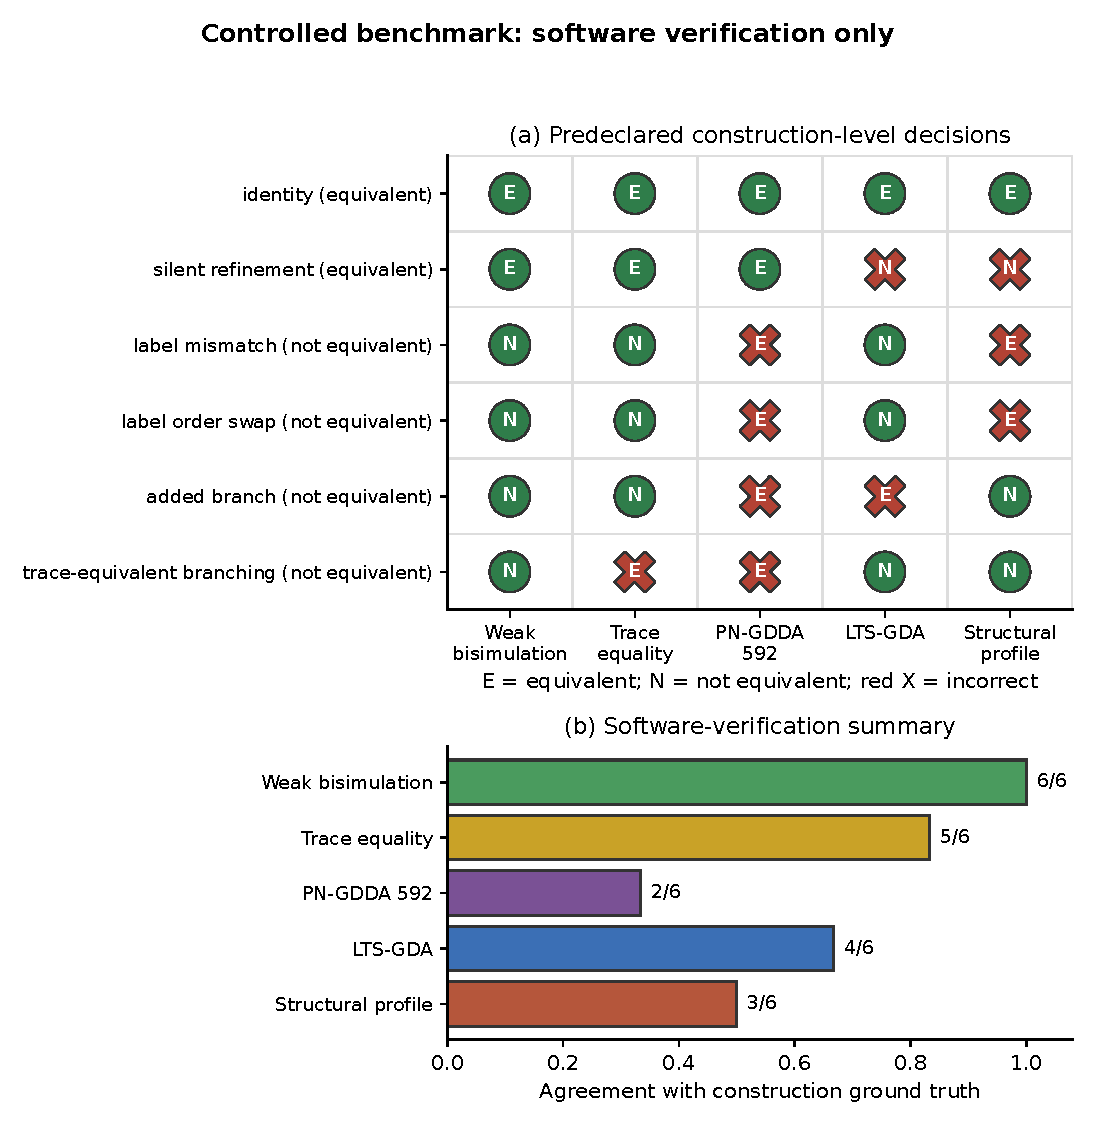
\includegraphics[width=\textwidth]{Fig3.pdf}
\caption{Controlled software/formal benchmark. (a) Decisions for six cases whose
labels were fixed by construction; a red cross marks disagreement with that
label. (b) Agreement count on this limited task. Trace equality loses branching;
PN-GDDA is label-blind; LTS-GDA retains local labels but does not abstract silent
refinement or recursively match successors. The panel verifies implementation
behavior and does not measure biological validity or generic method superiority.}
\label{fig:benchmark}
\alttext{A benchmark heatmap and bar chart comparing five methods on six
controlled model pairs.}
\end{figure}

The structural profile averages state-count, edge-count, label-multiset, and
out-degree-multiset similarities. The trace diagnostic declares a depth-$8$
match when $d_8=0$. PN-GDDA was implemented from its published definition using
151 directed bipartite graphlets and the 592 published/Holmes orbit
slots.\cite{Szawulak2022} For orbit $j$,
\begin{equation}\label{eq:pn-gdda}
N_G^j(k)=\frac{D_G^j(k)/k}{\sum_{r>0}D_G^j(r)/r},\quad
A^j(G,H)=1-\frac{\left[\sum_k(N_G^j(k)-N_H^j(k))^2\right]^{1/2}}{\sqrt{2}},
\end{equation}
and PN-GDDA is the mean $A^j$. Synthetic LTSs use an exact state-machine Petri
net encoding; curated pairs use their native nets. The 0.9 threshold is a fixed
diagnostic decision, not an equivalence relation. LTS-GDA instead combines four
reachable-graph orbits with labeled edge, two-step, divergence, and convergence
motifs.

The catalog audit recovered 151 graphlets and 592 slots from hash-verified Holmes
1.1.1/2.0.1.2 JARs. A direction- and type-preserving automorphism partition has
576 distinct orbits; using it is reported only as sensitivity. A Java probe
matched every Holmes 1.1.1 topology/root assignment. On a four-node test net and
its one-arc deletion, Python and Holmes scores were 0.9872027465870733 and
0.987202746587073, agreeing to 12 decimal places. Holmes is an independent
software reference for the structural score.\cite{Radom2017}

\subsection{Independent formal oracles}\label{sec:mcrl2-method}

Each analyzed LTS was exported in Aldebaran AUT format and evaluated with
\texttt{ltscompare} from hash-pinned mCRL2 202607.0.\cite{Bunte2019} The tool
independently checked strong bisimilarity, weak bisimilarity, and exact weak-trace
equivalence with \texttt{tau} hidden. Its used interface does not expose the weak
simulation preorder, so no one-way simulation is attributed to mCRL2.

A separately coded attacker--defender game grows the least set of positions from
which an unmatched move can be forced. It agreed with the production simulation
algorithm on all 67,600 ordered pairs among all 260 one- and two-state LTSs over
$\{a,\TAU\}$. This is exhaustive within that finite universe, not a proof for
arbitrary systems. Across the six synthetic pairs, six public-model controls,
and nine HPN comparisons below, Python and mCRL2 agreed on all 42 reported
strong/weak decisions. Theorem~\ref{thm:fixed-point}, finite exhaustive testing,
and external-tool comparison are distinct evidence layers.

\subsection{Observed computational scaling and reproducibility}
\label{sec:scalability-method}

Linear workflows of 8, 16, 32, 64, 96, and 128 transitions were compared with an
identity and a silently refined copy. Median runtime over three repetitions rose
from about 0.4 ms for nine states to about 0.6 s for the largest pairs. The
128-step identity relation had 16,641 candidate pairs; refinement increased it
to 18,705 pairs over 129 and 145 states. Every class remained as constructed
(the complete plot and table are archived in the repository). Timings used
Python 3.11.8 on an Apple M3 Pro with 18 GiB memory and are machine-dependent.

The Python standard library implements reachability, formal relations, parsers,
and controlled models. NumPy, pandas, Matplotlib, NetworkX, pydot, and Graphviz
support tabulation and figures. Fixed seeds, source hashes,
machine-readable outputs, unit tests, an executed notebook, environment files,
and continuous integration are public. Runtime CSV values are excluded from
byte-level regression because they depend on hardware; all scientific outcomes
and other result tables are deterministic.

\section{Biological network applications}
\label{sec:applications}

\subsection{Biological question and observational-interface principles}
\label{sec:gim-question}

The central question is whether the animal/human and \tas{} DNA-damage models
encode a common executable control organization, and at which observational
resolution that correspondence ceases to hold. Independent biology supports
comparing broad functions but also requires preserving mechanistic distinctions.
ATM- and ATR-associated sensing, checkpoint control, repair, and recovery occur
in both kingdoms; mammalian p53/apoptosis and the plant-specific SOG1, WEE1, SMR,
and damage-associated endoreduplication programs are not interchangeable
mechanisms.\cite{JacksonBartek2009,BlackfordJackson2017,Yoshiyama2013,
DeSchutter2007,Yi2014,Adachi2011,Ogita2018,ManovaGruszka2015}

We therefore evaluated three biologically motivated interfaces on exactly the
same two Petri-net structures and initial markings. Interface A observes five
coarse functions: damage detection, checkpoint activation, repair, restoration,
and exit from the proliferative cycle. Interface B additionally distinguishes
double-strand-break and replication-stress detection, ATM- and ATR-associated
signaling, and broad repair families, while retaining a common terminal
\texttt{cell\_cycle\_exit} readout. Interface C preserves those distinctions and
separately exposes mammalian \texttt{apoptosis}, plant
\texttt{smr\_induction}, and the plant net's combined
\texttt{differentiation\_or\_endoreduplication} transition. The last label is a
property of this compact encoding: the model does not infer differentiation and
endoreduplication as separate branches. Table~\ref{tab:gim-interface-rationale}
records why each process is observed or hidden. The executable definitions and
the literature keys were fixed in source data and are exported as a
machine-readable audit table.

\begin{table}[t]
\tbl{Biological rationale for the GIM observational interfaces. ``A'' denotes
coarse function; ``B/C'' denotes the pathway-resolved interfaces.
\label{tab:gim-interface-rationale}}{
\begin{tabular}{@{}>{\raggedright\arraybackslash}p{0.70in}%
>{\raggedright\arraybackslash}p{1.10in}%
>{\raggedright\arraybackslash}p{1.10in}%
>{\raggedright\arraybackslash}p{1.65in}@{}}
\toprule
Process & Animal/human encoding & \tas{} encoding & Interface treatment and
independent support \\
\colrule
Damage sensing & ATM-dominant DSB and ATR-dominant replication-stress channels
& ATM/ATR channels upstream of SOG1 & A merges detection; B/C distinguish the
initiating channels. \cite{BlackfordJackson2017,Yoshiyama2013,Adachi2011} \\
Checkpoint & CHK1/2--p53--p21 control & SOG1-regulated WEE1 and SMR
control & A exposes function; B/C expose ATM/ATR but keep downstream relays
internal. \cite{JacksonBartek2009,DeSchutter2007,Yi2014,Ogita2018} \\
Repair & DSB and excision-repair families followed by recovery & Broad
DSB and excision-repair families followed by recovery & A merges repair; B/C
separate repair families. \cite{JacksonBartek2009,ManovaGruszka2015,
Yoshiyama2013} \\
Unresolved damage & Apoptotic exit from the proliferative pool & SMR-associated
arrest followed by a combined differentiation/endoreduplication outcome & A/B
collapse terminal loss; C distinguishes encoded mechanisms.
\cite{JacksonBartek2009,Yi2014,Adachi2011,FulcherSablowski2009} \\
\botrule
\end{tabular}}
\end{table}

\subsection{GIM: encoded DNA-damage control across observational resolutions}
\label{sec:gim-results}

The animal and plant nets reach 13 and 14 states, respectively. Because only
transition labels change across interfaces, their native PN-GDDA structural
similarity remains 0.9975846 (0.9975175 with the independently derived 576-orbit
partition). This high value says that the selected Petri-net wiring is similar;
it says nothing about labels, initial states, or reachable branching.

At Interface A the two LTSs are weakly, but not strongly, bisimilar: every
displayed detection--checkpoint--repair path and each restoration or cycle-exit
branch can be matched after internal relays are hidden. The result persists at
Interface B, so separating damage, ATM/ATR, and repair channels does not by
itself break the relation in these encodings. At Interface C, however, weak
bisimilarity and both simulation directions fail. The truncated-trace distance
changes from $d_6=0$ at A and B to $d_6=0.3529$ at C, while LTS-GDA falls from
0.9508 to 0.8921 (Table~\ref{tab:gim-sensitivity}). The structural score is
unchanged because no place, transition, or arc was altered.

\begin{figure}[t]
\centering
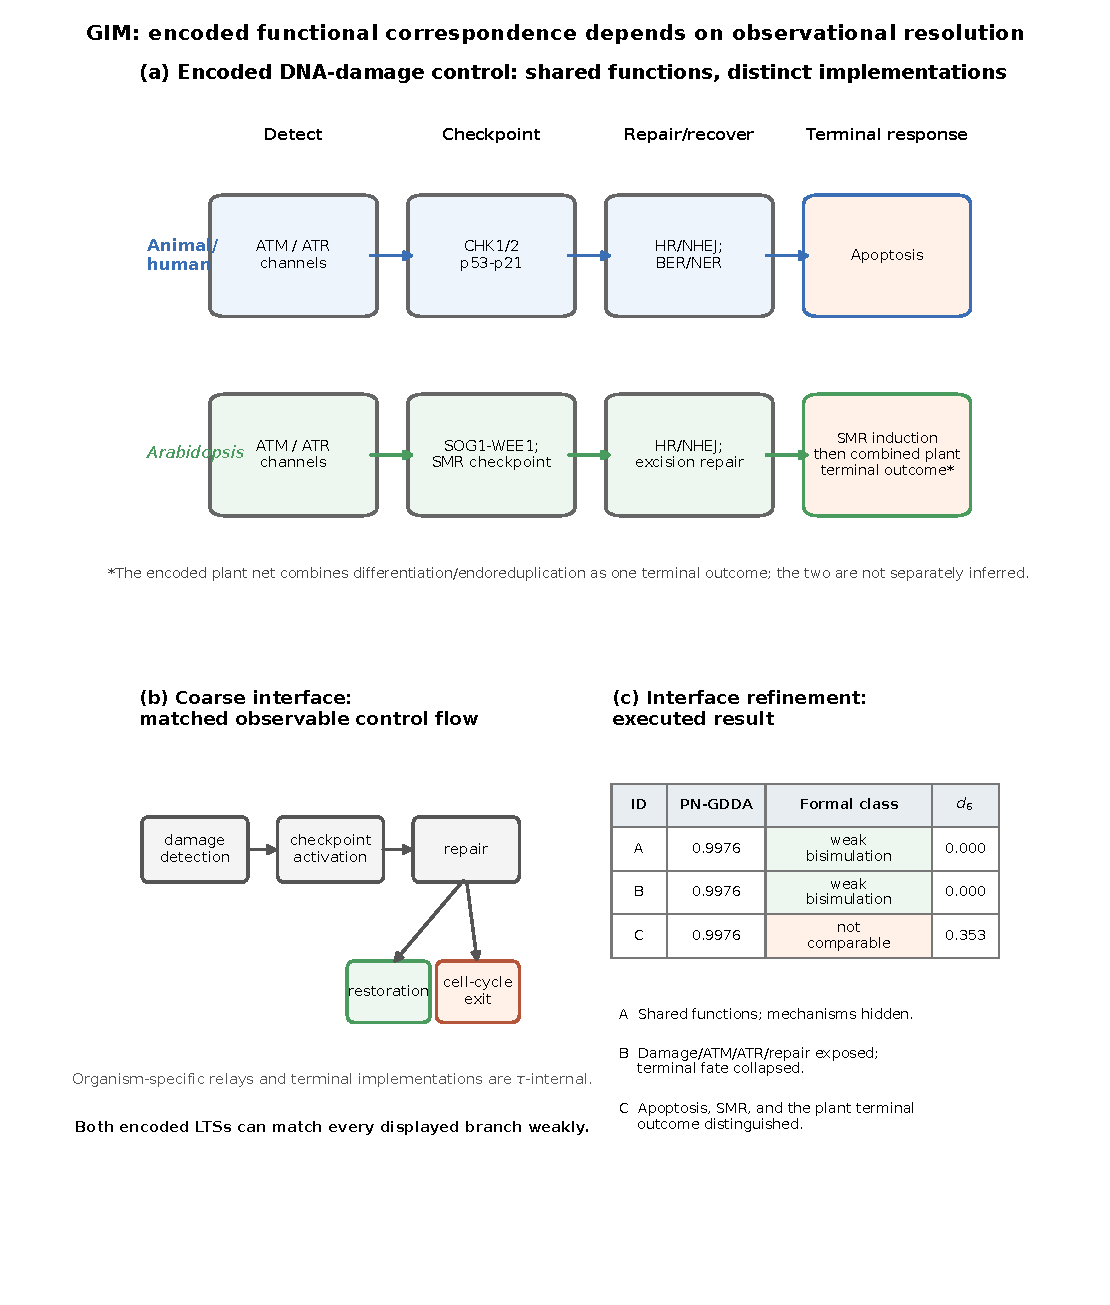
\includegraphics[width=\textwidth]{Fig2.pdf}
\caption{Central GIM case study. (a) The encoded models share broad
damage-response functions but use distinct regulatory and terminal mechanisms.
(b) At the coarse interface, both reachable LTSs match the displayed branching
after organism-specific relays are hidden. (c) Executed sensitivity analysis:
Interfaces A and B are weakly bisimilar, whereas Interface C is non-comparable
when terminal mechanisms are separate observations. PN-GDDA remains 0.9976
because the Petri-net structures do not change. These are model- and
interface-conditional results, not organism-level equivalence.}
\label{fig:gim-interface}
\alttext{Three panels compare animal and Arabidopsis DNA-damage functions,
coarse observable control flow, and formal results under three interfaces.}
\end{figure}

\begin{table}[t]
\tbl{Executed GIM interface-sensitivity analysis. A$\preceq$P means that the
animal-model behavior is weakly simulated by the plant model; P$\preceq$A is
the reverse direction. Strong bisimulation was false for all three interfaces.
\label{tab:gim-sensitivity}}{
\begin{tabular}{@{}lp{1.75in}ccp{1.15in}rr@{}}
\toprule
ID & Observational resolution & A$\preceq$P & P$\preceq$A & Formal class & $d_6$ & PN-GDDA \\
\colrule
A & Coarse functional/process & Y & Y & weak bisimulation & 0.0000 & 0.9976 \\
B & Damage/signaling/repair pathways; terminal fate collapsed & Y & Y & weak bisimulation & 0.0000 & 0.9976 \\
C & Mechanism-resolved terminal fate & N & N & not comparable & 0.3529 & 0.9976 \\
\botrule
\end{tabular}}
\end{table}

The comparison thus contributes information unavailable from structure alone:
it locates the observational boundary of the encoded correspondence. The A/B
result is consistent with shared high-level damage-response functions, but does
not identify p53 with SOG1 or plant terminal responses with apoptosis. The C
result reflects the known distinction between these mechanisms and shows that
the apparent correspondence depends on collapsing them into a common functional
outcome. A limited model-derived hypothesis follows: assays or model readouts
that aggregate terminal loss of proliferative capacity should be more compatible
with the A/B correspondence, whereas readouts distinguishing apoptosis, SMR
induction, and differentiation/endoreduplication should break it. This is a
testable consequence of the two encodings, not an experimentally established
cross-organism claim. Full Petri-net diagrams are retained in
Appendix~\ref{app:gim-nets}.

\subsection{Cross-format ingestion and execution controls}
\label{sec:public-method}

Two externally authored GINsim models test the complete import-to-comparison
path: the 13-component mammalian cell cycle in SBML-qual and the four-component
multilevel p53--Mdm2 model in GINML.\cite{Naldi2018,Traynard2016,
Chaouiya2013SBML,AbouJaoude2009} Files, URLs, and SHA-256 values are archived.
Unitary-asynchronous updates move one enabled component by one level and label
its direction. Each base model was compared with an exact copy, five silent
subdivisions, and a reachable-label perturbation. All six controls recovered
their predeclared strong/weak/exact-trace outcomes in Python and mCRL2
(Table~\ref{tab:public-controls}).

\begin{table}[t]
\tbl{Public GINsim models and control outcomes. S/W/T denote strong, weak, and
exact weak-trace equivalence.\label{tab:public-controls}}{
\begin{tabularx}{\textwidth}{@{}p{0.25\textwidth}lrrccc@{}}
\toprule
Model & Format & States & Edges & Copy & Silent & Perturbed \\
\colrule
Mammalian cell cycle & SBML-q & 826 & 3,413 & Y/Y/Y & N/Y/Y & N/N/N \\
p53--Mdm2 damage & GINML & 17 & 26 & Y/Y/Y & N/Y/Y & N/N/N \\
\botrule
\end{tabularx}}
\end{table}

Synchronous execution reached 13 of 826 asynchronous cell-cycle states (Jaccard
0.0157) and eight of 17 p53--Mdm2 states (Jaccard 0.471), confirming sensitivity
to update semantics. These are cross-format execution controls, not biological
validation.

\subsection{Exploratory HPN-DREAM/CASPOTS held-out analysis}\label{sec:hpn-method}

The public HPN-DREAM phosphoproteomic series and CASPOTS Boolean families contain
72 BT20, 191 BT549, and 21 MCF7 networks.\cite{Hill2016,Razzaq2018} One
representative per cell line was selected before test responses were read: the
model with maximum mean within-family Jaccard similarity between active clauses,
with exact lexicographic tie-breaking. This structure-only rule selected
zero-based rows 24, 137, and 9 (Table~\ref{tab:hpn-medoids}); an anti-leakage test
forbids access to test files during selection.

\begin{table}[t]
\tbl{HPN-DREAM families and structure-only representatives.
\label{tab:hpn-medoids}}{
\begin{tabular}{@{}lrrrr@{}}
\toprule
Cell line & Family & Medoid row$^a$ & Clauses & Mean Jaccard \\
\colrule
BT20  & 72  & 24  & 29 & 0.815 \\
BT549 & 191 & 137 & 25 & 0.854 \\
MCF7  & 21  & 9   & 23 & 0.851 \\
\botrule
\end{tabular}}
\begin{tabnote}$^a$Zero-based row; selected from model structure only.\end{tabnote}
\end{table}

The interface is the intersection of seven measured PI3K/MAPK/mTOR readouts.
The three common test perturbations are mTOR inhibition, IGF1 plus mTOR
inhibition, and 4EBP1 plus mTOR inhibition. Measured time-zero values initialize
readouts; stimuli and inhibitors are clamped; other relevant nodes start at zero.
Primary asynchronous LTSs label interface updates and hide all others. The nine
cross-cell pair-condition comparisons were repeated synchronously; this stress
test is not a most-permissive analysis. CASPOTS itself evaluates asynchronous
trajectories.\cite{Pauleve2020,Razzaq2018}

Experimental distance is RMSE over common post-zero times and readouts. Spearman
associations use an exact one-sided permutation of the three cell-pair labels
within each condition ($3!^3=216$). CASPOTS/Clingo compatibility scores consume
optimization to completion, use deterministic secondary tie-breaks, and were
reproduced twice. Native specificity uses the exact sign permutation of three
native-minus-mean-cross differences.

Selected LTSs had 2--44 states. None of the nine cross-cell pairs was weakly
bisimilar: six had one-way simulation and three were not comparable. Direction
was retained explicitly, with three left-model-in-right-model and three
right-model-in-left-model relations. These categories do not form a justified
one-dimensional order, and the held-out RMSE is symmetric between each cell
pair. We therefore removed the former ordinal class coding and performed no
scalar formal-class test. Descriptively, median RMSE was 0.2418 for the six
one-way relations and 0.2071 for the three non-comparable pairs; after preserving
direction, the corresponding medians were 0.2757, 0.1919, and 0.2071, each based
on only three observations. These summaries are not inferential evidence.

The two predeclared continuous diagnostics were retained. Truncated-trace
distance gave $\rho=-0.596$ (exact one-sided $p=0.556$), and LTS-GDA distance
gave $\rho=0.669$ ($p=0.097$) under 216 condition-stratified permutations.
Neither association is conclusive. Synchronous updating preserved seven of nine
formal classes.

Native medoid RMSE was 0.33024 (BT20), 0.31335 (BT549), and 0.27726 (MCF7),
against discretization RMSE 0.32944, 0.30079, and 0.27726. Native excess-RMSE
advantage over mean cross-cell medoids was 0.00212 and not established by the
exact sign test ($p=0.25$; Fig.~\ref{fig:hpn-validation}). The result demonstrates
an exploratory held-out compatibility check and separates formal similarity
from empirical response similarity; it does not demonstrate cell-line
specificity or predictive discrimination.

\begin{figure}[t]
\centering
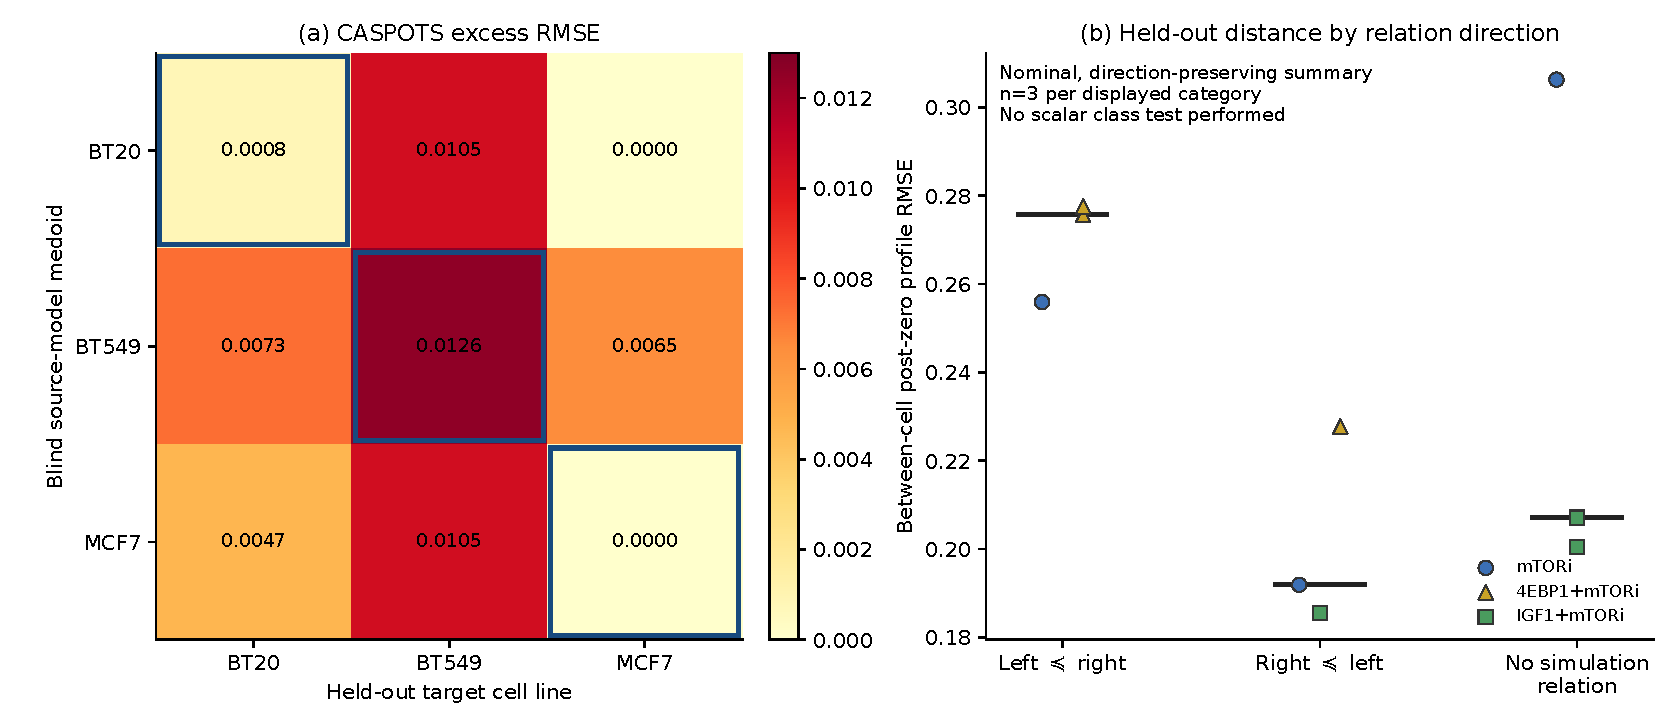
\includegraphics[width=\textwidth]{Fig8.pdf}
\caption{Exploratory held-out HPN-DREAM analysis. (a) CASPOTS excess RMSE by
source medoid and target; outlined cells are native contexts. (b) Between-cell
profile RMSE with the direction of weak simulation retained. Horizontal bars
are medians; each category has $n=3$, and no scalar formal-class test was
performed. Neither panel establishes native cell-line specificity.}
\label{fig:hpn-validation}
\alttext{CASPOTS excess-error matrix and a direction-preserving nominal display
of held-out response distances for three breast-cancer cell lines.}
\end{figure}

\subsection{Secondary curated comparisons}\label{sec:case-method}

Five compact plant--animal pairs encode DNA repair/genome instability (GIM), energy
metabolism (DCE), cell-cycle control (SPS), cell death/autophagy (RCD), and
immune control (AID). Comparative studies and cancer-hallmark literature guided
component selection; dedicated reviews informed plant DNA-damage, cell-cycle,
and autophagy mechanisms.\cite{Quimbaya2012,ClavijoBuritica2023,Hanahan2022,
Yoshiyama2013} Transition-level provenance is machine-checked, which establishes
where encoded assumptions came from and whether documentation is complete. It
does not establish that the nets reproduce independent experiments. These
manually curated models contain no kinetics, concentrations, tissue context, or
independent experimental calibration.

The ten nets produced 5--14 reachable states. The GIM row in
Table~\ref{tab:case} reports Interface A; GIM, DCE, and SPS were weakly but
not strongly bisimilar; RCD gave plant-in-animal one-way simulation; AID was
non-comparable. Table~\ref{tab:case} juxtaposes these classes with native
PN-GDDA. The 592- and 576-orbit variants changed no score by 0.001 and no
threshold decision: all five pairs were structurally similar at 0.9 despite
three different behavioral classes.

\begin{table}[t]
\tbl{Supporting curated model-pair outputs. GIM is reported at Interface A;
all relations and $d_6$ values are interface-conditional, whereas PN-GDDA is
structural.\label{tab:case}}{
\begin{tabular}{@{}l>{\raggedright\arraybackslash}p{1.05in}>{\raggedright\arraybackslash}p{1.05in}rrr@{}}
\toprule
Module & Process & Formal class & $d_6$ & PN-592 & Orbit-576 \\
\colrule
GIM & DNA repair & weak bisimulation & 0.000 & 0.9976 & 0.9975 \\
DCE & energy metabolism & weak bisimulation & 0.000 & 0.9969 & 0.9968 \\
SPS & cell-cycle control & weak bisimulation & 0.000 & 1.0000 & 1.0000 \\
RCD & death/autophagy & plant in animal & 0.143 & 1.0000 & 1.0000 \\
AID & immune control & non-comparable & 0.429 & 0.9907 & 0.9904 \\
\botrule
\end{tabular}}
\end{table}

RCD supplies a secondary directional result: both encoded nets contain stress,
mTOR inhibition, autophagy, and survival, but only the animal encoding exposes a
canonical caspase-apoptosis branch; the plant branch uses an internal metacaspase
event. The plant LTS is weakly simulated by the animal LTS, whereas the reverse
direction fails. This means containment only for the declared labels of these
two models; it does not equate plant programmed cell death with mammalian
apoptosis. Silent subdivision preserved every class over 300 refinements per
module, while targeted relabeling changed the expected relations. Distances
against 2,000 label permutations assess internal interface sensitivity, not
external biological significance. DCE, SPS, and AID are retained as supporting
model-ingestion and relation-diversity examples rather than independent
biological validation.

\section{Discussion}\label{sec:discussion}

\subsection{Structural and behavioral correspondence}
\label{sec:discussion-meaning}

The classifier turns an ordered pair of executable models into one statement at
a declared observational interface. Proposition \ref{prop:hierarchy} supports
the reporting priority: strong bisimilarity entails weak bisimilarity, and weak
bisimilarity entails both simulation directions. One-way classes retain their
orientation and therefore express behavioral containment, not equivalence. The
fixed-point theorem concerns the algorithm actually executed, including its
in-place deletion order and treatment of $\TAU$; software tests complement that
proof but cannot replace it.

The controlled cases show why structural, linear-time, and branching
comparisons answer different questions. Identical unlabeled structure cannot
determine labeled behavior (Proposition \ref{prop:label-blind}), while Example
\ref{ex:branching} has identical exact finite traces but different branching.
PN-GDDA agreed with 2/6 construction-level behavioral labels even though the
independent Holmes implementation reproduced every structural score to 12
decimal places. This is not a defect in PN-GDDA: labels, initial states, and
reachable branching are outside that statistic by design. Similarly, LTS-GDA
retains labeled local motifs but does not perform silent abstraction or
recursive successor matching.

GIM makes that complementarity biologically interpretable. Its structural score
remains 0.9976 under all three interfaces, while the behavioral class changes
from weak bisimulation to non-comparability only when terminal mechanisms become
observable. The structural result describes similar selected wiring; the
behavioral result describes what the reachable models can match under a
biological readout. Neither statement subsumes the other.

\subsection{Interface and update semantics}
\label{sec:discussion-interface}

Every relation is indexed by $\Sigma$. Declaring an event internal changes the
paths hidden by abstraction, while merging outcomes under one label coarsens the
question. In GIM, A and B collapse apoptosis and the encoded plant terminal
sequence into \texttt{cell\_cycle\_exit}; their weak bisimilarity consequently
means agreement only at that functional resolution. Interface C separates those
events and is non-comparable in both simulation directions. The interface is
therefore a falsifiable modeling assumption, not a post-processing convenience.
Proposition \ref{prop:silent-refinement} covers the controlled transition
subdivisions used here, but not refinements that introduce conflicts,
interleavings, or observable choices.

Update semantics is likewise part of the comparison contract. Switching between
asynchronous and synchronous execution changed public GINsim behavior and two HPN
classes. General-asynchronous, most-permissive, and stochastic conventions were
not evaluated.\cite{Pauleve2020} A reported relation should therefore always name
both its observable interface and execution semantics.

\subsection{Evidence and biological limits}
\label{sec:discussion-biological}

Table~\ref{tab:evidence-layers} separates four claims that are otherwise easy to
conflate. Layer I is mathematical. Layer II asks whether the implementation
computes the declared objects: Python and mCRL2 agreed on all 42 strong/weak
decisions, and the independent game agreed on all 67,600 ordered pairs in its
complete two-state universe. Layer III concerns the executable biological
models. Hashes, parser controls, and transition provenance make ingestion and
assumptions reproducible, but do not show that a model reproduces biology.
Layer IV concerns independent biological support. The GIM interpretation is
consistent with literature on shared functions and distinct mechanisms, but its
interface-dependent relation remains derived from curated models; its assay
consequence is a hypothesis. HPN supplies held-out measurements, but only nine
pair--condition observations and no conclusive inferential result.

\begin{table}[t]
\tbl{Evidence taxonomy used for claims in this study.
\label{tab:evidence-layers}}{
\begin{tabular}{@{}>{\raggedright\arraybackslash}p{0.62in}%
>{\raggedright\arraybackslash}p{1.25in}%
>{\raggedright\arraybackslash}p{1.30in}%
>{\raggedright\arraybackslash}p{1.35in}@{}}
\toprule
Layer & Evidence used here & What it supports & What it does not establish \\
\colrule
I Formal & Definitions, propositions, fixed-point proof, finite
termination & Correctness of the stated mathematics and executed relation
operator & Correct software or biological relevance by itself \\
II Software & Six constructed cases, mCRL2, independent game,
regression tests & Recovery of declared formal distinctions in tested domains &
Biological usefulness or empirical validity \\
III Model & Hash-pinned GINsim files, parser controls,
transition provenance, explicit semantics & Reproducible origin, ingestion, and
assumptions of the encoded models & Experimental calibration or faithful
organism-level behavior \\
IV Biological & Independent DDR literature; exploratory
HPN-DREAM/CASPOTS responses & Biological plausibility and a route for confronting
formal outputs with data & Confirmed cross-organism equivalence, prognosis, or
cell-line specificity \\
\botrule
\end{tabular}}
\end{table}

The HPN limitations are substantive rather than presentational. Directional
simulation relations do not define an ordinal scale, so assigning them scalar
ranks would discard their meaning; the revised analysis reports the directions
nominally and makes no class-level inferential test. The retained trace and
LTS-GDA associations are inconclusive, and the CASPOTS native-versus-cross
advantage is not established ($p=0.25$). CASPOTS RMSE is minimum-distance
compatibility over admissible trajectories, not a unique time-series
prediction.\cite{Razzaq2018} These observations do not support prognostic or
cell-line-specific claims.

The curated Petri nets additionally omit kinetics, concentrations, stochastic
effects, tissue context, and independent experimental calibration. Provenance
establishes why a transition was included and whether its documentation is
complete; it is not model validation or validation of a biological conclusion.
Label-permutation results measure sensitivity within those constructions, and
cross-organism weak relations never imply organism-level functional identity.

\subsection{Computational scope and use}
\label{sec:discussion-computation}

The implementation explicitly enumerates states and may store
$|S_1||S_2|$ candidate pairs. The scaling experiment reached 145 states and
18,705 pairs, so it does not establish genome-scale performance. Symbolic state
representations, partition refinement, and compositional checking are natural
extensions. PN-GDDA was applied to native curated nets and canonical
state-machine encodings; using it on SBML-qual or Boolean rules would require a
non-unique reverse translation. Larger repository models, prospectively
expert-labeled relations, biological replicates, blinded interface selection,
and additional update semantics are required before broader predictive claims.
At present, the framework is best used to audit two explicit qualitative models
at a predeclared observational resolution.

\section{Conclusion}\label{sec:conclusion}

Comparing executable qualitative biological models requires an explicit account
of observables, silent events, initial states, branching, and update semantics.
The classifier reports the strongest supported relation from strong
bisimilarity through directional weak simulation, with fixed-point correctness
and termination established for finite LTSs. Controlled cases, mCRL2, and the
independent game verify distinct parts of the implementation; they are not
biological validation.

In the unchanged GIM Petri-net structures, PN-GDDA remained 0.9976 while the
behavioral relation changed with observational resolution. Coarse function and
pathway-resolved interfaces were weakly bisimilar, but exposing mammalian
apoptosis and the encoded plant SMR--differentiation/endoreduplication sequence
made the models non-comparable in both directions. The useful conclusion is not
that behavioral comparison is generically superior to structural comparison,
but that the two expose complementary properties and that an explicit interface
locates where apparent model correspondence breaks. Public-model controls and
the exploratory HPN analysis show how the audit crosses formats and can be
confronted with data, while the inconclusive HPN statistics delimit current
evidence. The framework supports reproducible, question-specific model auditing;
it does not establish prognosis, cell-line specificity, mechanistic identity, or
organism-level equivalence.

\appendix
\section{Detailed GIM Petri-net encodings}\label{app:gim-nets}

Figures~\ref{fig:gim-animal-net} and \ref{fig:gim-plant-net} retain the full
executable diagrams underlying the biological schematic and all three interface
analyses. The place/transition structures and initial markings are fixed;
interface-specific labels are assigned reproducibly by
\texttt{gim\_models\_for\_interface}.

\clearpage
\begin{sidewaysfigure}[p]
\centering
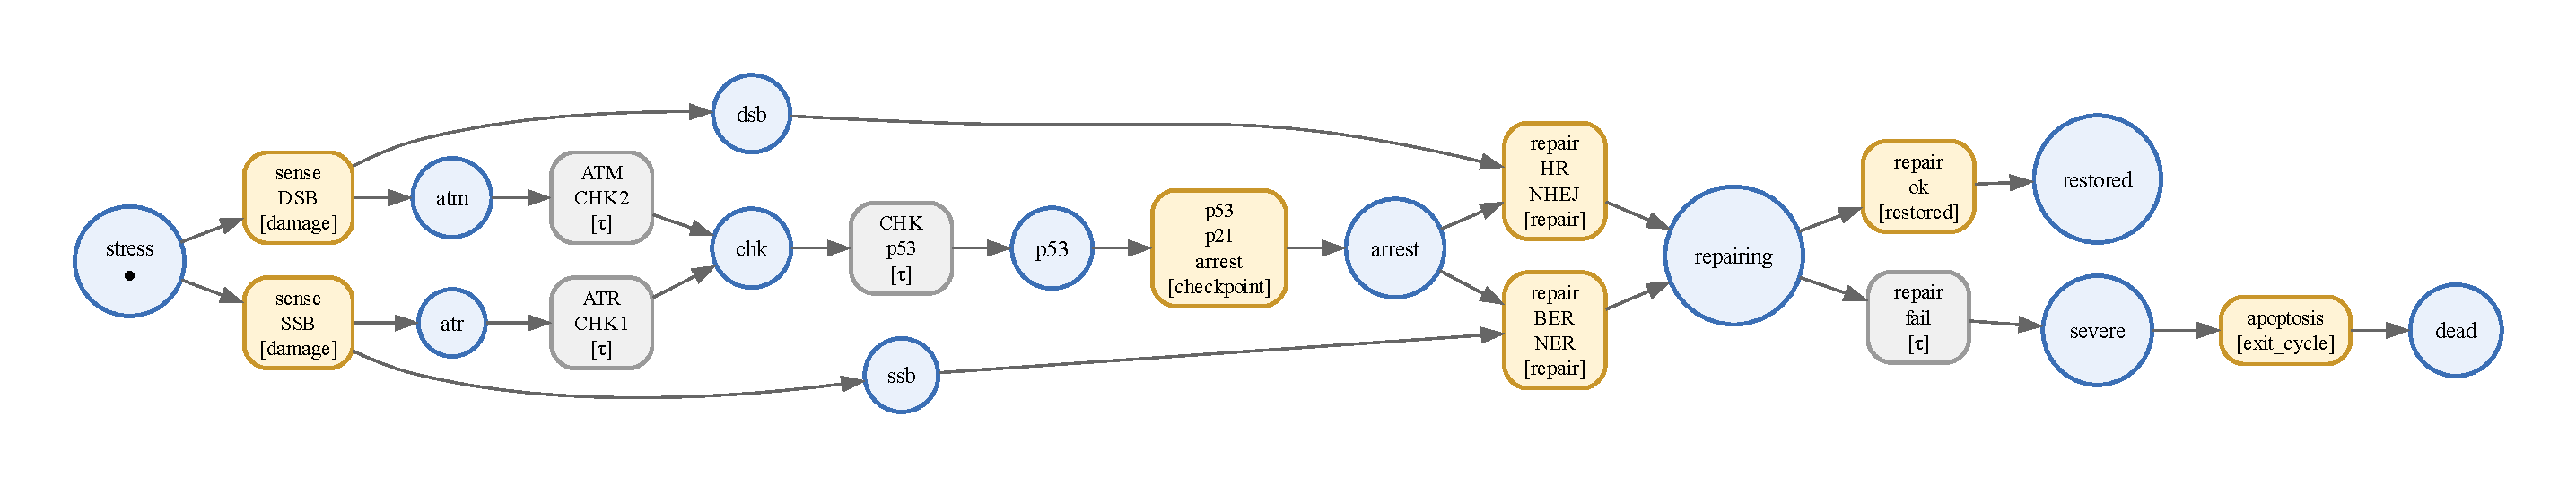
\includegraphics[width=0.94\textheight]{FigS1a.pdf}
\caption{Detailed animal/human GIM Petri net. Circles are places, rounded boxes
are transitions, brackets show the base/coarse observable labels, and gray
$\tau$ transitions are internal.}
\label{fig:gim-animal-net}
\alttext{Detailed animal and human DNA-damage Petri net with places,
transitions, labels, and arcs.}
\end{sidewaysfigure}

\begin{sidewaysfigure}[p]
\centering
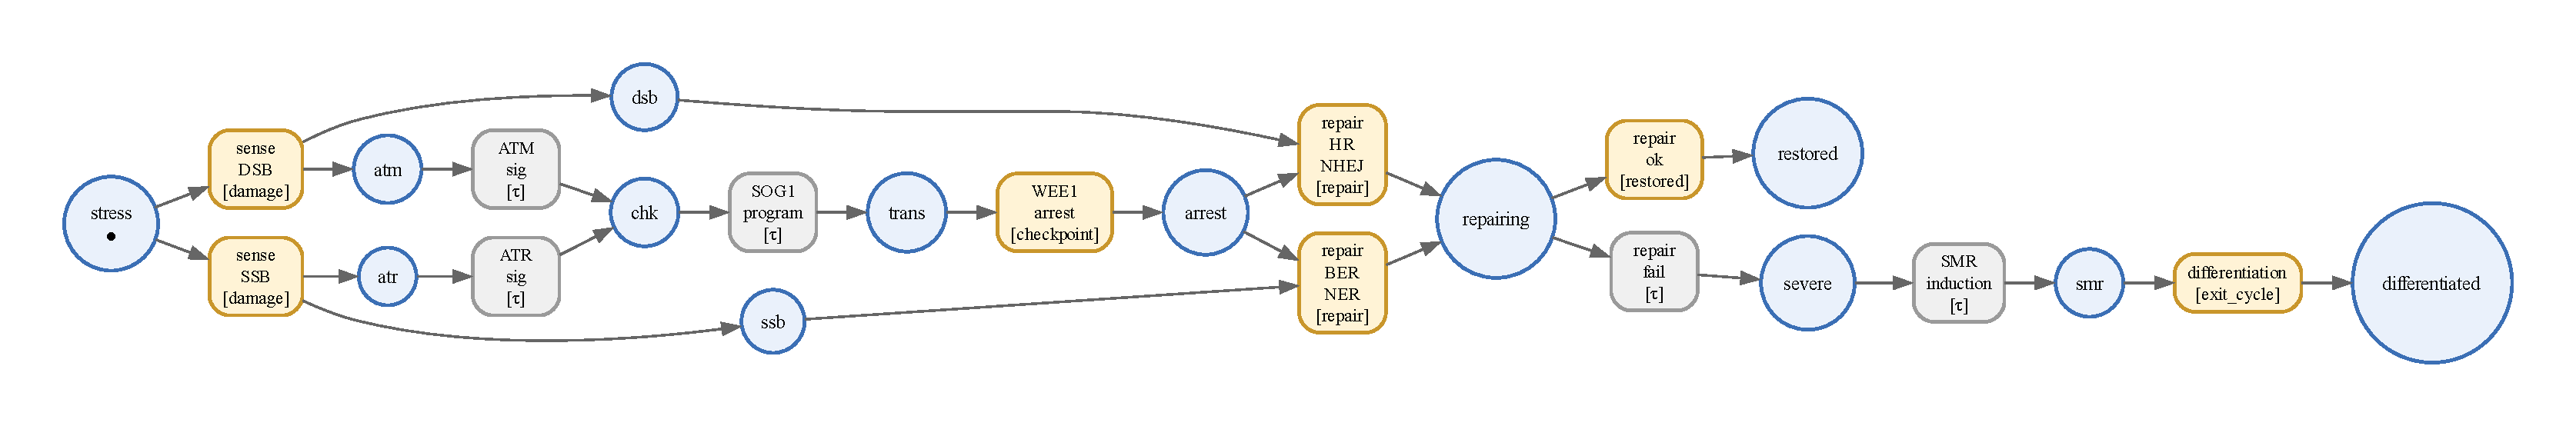
\includegraphics[width=0.94\textheight]{FigS1b.pdf}
\caption{Detailed \tas{} GIM Petri net, using the same graphical conventions as
Fig.~\ref{fig:gim-animal-net}. The terminal transition is a combined outcome in
this encoding and does not distinguish differentiation from endoreduplication.}
\label{fig:gim-plant-net}
\alttext{Detailed Arabidopsis DNA-damage Petri net with places, transitions,
labels, and arcs.}
\end{sidewaysfigure}

\clearpage

\section*{Data and code availability}

Code, curated definitions, hash-verified public models, normalized response
files, metadata, and generated results are available under the MIT License at
\url{https://github.com/cero1979/BisimulationMol}. The repository documents
formal/software verification, interface definitions, figure regeneration,
tests, and notebook execution. Machine-readable GIM and HPN results are provided
as \texttt{results/gim\_interface\_sensitivity.csv} and
\texttt{results/hpn\_dream\_formal\_data\_validation.csv}. No confidential or
participant-level data were used.

\section*{Declarations}

\noindent\textbf{Funding.} No specific funding was received.
\textbf{Competing interests.} The author declares no competing interests.
\textbf{Ethics.} Only computational models and published aggregate data were
used; no human participants, samples, or live animals were involved.
\textbf{Author contributions.} Carlos Ramirez Ovalle performed the
conceptualization, methodology, software, formal analysis, validation,
visualization, drafting, and revision.

\input{bibliography_jbcb.bbl}

\end{document}
